\documentclass[11pt,a4paper]{article}

% ==============================================================================
% PACKAGES & THEME CONFIGURATION
% ==============================================================================
\usepackage[utf8]{inputenc}
\usepackage[T1]{fontenc}
\usepackage{lmodern}
\usepackage[margin=1.8cm,top=2.2cm,bottom=2.2cm]{geometry}
\usepackage{microtype}
\usepackage{xcolor}
\usepackage{amsmath,amssymb}
\usepackage{booktabs}
\usepackage{tabularx}
\usepackage{array}
\usepackage{enumitem}
\usepackage{titlesec}
\usepackage{fancyhdr}
\usepackage{lastpage}
\usepackage{tikz}
\usetikzlibrary{shapes.geometric,arrows.meta,positioning,calc,fit,backgrounds}
\usepackage[most]{tcolorbox}
\usepackage{listings}
\usepackage[hidelinks,colorlinks=true,linkcolor=brandblue,citecolor=brandteal,urlcolor=brandblue]{hyperref}

% ==============================================================================
% COLOR PALETTE (Modern Corporate Tech Theme)
% ==============================================================================
\definecolor{brandnavy}{HTML}{0F172A}      % Slate 900
\definecolor{brandslate}{HTML}{1E293B}     % Slate 800
\definecolor{brandblue}{HTML}{0284C7}      % Sky 600
\definecolor{brandteal}{HTML}{0D9488}      % Teal 600
\definecolor{brandemerald}{HTML}{059669}   % Emerald 600
\definecolor{brandamber}{HTML}{D97706}     % Amber 600
\definecolor{brandrose}{HTML}{E11D48}      % Rose 600
\definecolor{bglight}{HTML}{F8FAFC}        % Slate 50
\definecolor{bgcode}{HTML}{F1F5F9}         % Slate 100
\definecolor{borderlight}{HTML}{CBD5E1}    % Slate 300
\definecolor{mutedgray}{HTML}{64748B}      % Slate 500

% ==============================================================================
% CODE LISTINGS STYLING
% ==============================================================================
\definecolor{pykeyword}{HTML}{0284C7}
\definecolor{pystring}{HTML}{059669}
\definecolor{pycomment}{HTML}{64748B}
\definecolor{pydecorator}{HTML}{D97706}
\definecolor{pyident}{HTML}{0F172A}

\lstdefinestyle{finforgestyle}{
    backgroundcolor=\color{bgcode},
    basicstyle=\ttfamily\footnotesize\color{brandnavy},
    keywordstyle=\bfseries\color{pykeyword},
    stringstyle=\color{pystring},
    commentstyle=\itshape\color{pycomment},
    numberstyle=\tiny\color{mutedgray},
    numbers=left,
    numbersep=8pt,
    frame=single,
    framerule=0.5pt,
    rulecolor=\color{borderlight},
    breaklines=true,
    breakatwhitespace=true,
    showstringspaces=false,
    tabsize=4,
    captionpos=b,
    xleftmargin=12pt,
    framexleftmargin=8pt
}

\lstdefinelanguage{yaml}{
    keywords={format_version, name, version, description, category, api_version, entrypoint, inputs, outputs, config, type, required, default, nodes, edges, id, component, source_node, source_port, destination_node, destination_port, metadata},
    keywordstyle=\bfseries\color{brandblue},
    sensitive=false,
    comment=[l]{\#},
    commentstyle=\itshape\color{mutedgray},
    stringstyle=\color{brandemerald},
    morestring=[b]',
    morestring=[b]"
}

\lstset{style=finforgestyle}

% ==============================================================================
% TCOLORBOX CALLOUT BOXES
% ==============================================================================
\newtcolorbox{calloutbox}[1][]{
    enhanced,
    colback=bglight,
    colframe=brandblue,
    leftrule=4pt,
    rightrule=0.5pt,
    toprule=0.5pt,
    bottomrule=0.5pt,
    arc=3pt,
    boxsep=5pt,
    fonttitle=\bfseries\color{brandnavy},
    coltitle=brandnavy,
    title={#1},
    attach boxed title to top left={yshift=-2mm, xshift=4mm},
    boxed title style={colback=white, colframe=brandblue, size=small, arc=2pt}
}

\newtcolorbox{alertbox}[1][]{
    enhanced,
    colback=bglight,
    colframe=brandamber,
    leftrule=4pt,
    rightrule=0.5pt,
    toprule=0.5pt,
    bottomrule=0.5pt,
    arc=3pt,
    boxsep=5pt,
    fonttitle=\bfseries\color{brandamber},
    title={#1},
    attach boxed title to top left={yshift=-2mm, xshift=4mm},
    boxed title style={colback=white, colframe=brandamber, size=small, arc=2pt}
}

\newtcolorbox{cheatsheetcard}[1]{
    enhanced,
    colback=bglight,
    colframe=brandnavy,
    leftrule=1pt,
    rightrule=1pt,
    toprule=1pt,
    bottomrule=1pt,
    arc=4pt,
    boxsep=6pt,
    coltitle=white,
    fonttitle=\bfseries\small,
    title={#1},
    colbacktitle=brandslate
}

% ==============================================================================
% HEADER & FOOTER
% ==============================================================================
\pagestyle{fancy}
\fancyhf{}
\renewcommand{\headrulewidth}{0.4pt}
\renewcommand{\footrulewidth}{0.4pt}
\fancyhead[L]{\textcolor{mutedgray}{\footnotesize \textbf{FinForge AI} --- Architecture, Cheat Sheet \& Roadmap}}
\fancyhead[R]{\textcolor{mutedgray}{\footnotesize Technical Reference Manual}}
\fancyfoot[L]{\textcolor{mutedgray}{\footnotesize Confidential \& Open-Source Architecture}}
\fancyfoot[R]{\textcolor{mutedgray}{\footnotesize Page \thepage\ of \pageref{LastPage}}}

% ==============================================================================
% SECTION HEADINGS FORMAT
% ==============================================================================
\titleformat{\section}
  {\Large\bfseries\color{brandnavy}}
  {\thesection}{1em}{}[\color{brandblue}\titlerule]

\titleformat{\subsection}
  {\large\bfseries\color{brandslate}}
  {\thesubsection}{1em}{}

\titleformat{\subsubsection}
  {\normalsize\bfseries\color{brandblue}}
  {\thesubsubsection}{1em}{}

% ==============================================================================
% DOCUMENT BEGIN
% ==============================================================================
\begin{document}

% ------------------------------------------------------------------------------
% TITLE BLOCK
% ------------------------------------------------------------------------------
\begin{center}
    {\fontsize{24pt}{28pt}\selectfont \textbf{\color{brandnavy}FinForge AI: Technical Architecture,}}\\[4pt]
    {\fontsize{18pt}{22pt}\selectfont \textbf{\color{brandblue}Master Cheat Sheet \& Strategic Roadmap}}\\[10pt]
    {\normalsize \textbf{Framework Version}: \texttt{0.1.0.dev0} \quad$|$\quad \textbf{Architecture Status}: Pre-Alpha Functional Foundation \quad$|$\quad \textbf{Language}: Python 3.11+}\\[6pt]
    \rule{\textwidth}{1.2pt}
\end{center}

\vspace{-6pt}
\begin{abstract}
\noindent \textbf{Executive Summary} --- Contemporary Artificial Intelligence and Machine Learning framework design is plagued by three fundamental engineering bottlenecks: \textit{opaque algorithmic black-boxes}, \textit{transitive dependency bloat}, and \textit{contract fragmentation}. \textbf{FinForge AI} is an open-source, general-purpose, modular AI framework architected around a strict \textbf{scratch-first} paradigm. By establishing standardized lifecycle state machines, zero-execution declarative manifests (\texttt{component.yaml}), static contract type verification, and directed acyclic graph (DAG) pipeline orchestration, FinForge AI enables practitioners, researchers, and financial engineers to implement algorithms from first principles and compose them into robust, reproducible, and verifiable production workflows. This document serves as the comprehensive architectural reference, implementation cheat sheet, and engineering roadmap for the FinForge AI framework.
\end{abstract}

\vspace{4pt}

% ------------------------------------------------------------------------------
% SECTION 1: THE CORE PHILOSOPHY
% ------------------------------------------------------------------------------
\section{The Core Philosophy: Why FinForge AI?}

\subsection{Dismantling the Wrapper-First Dilemma}
Over the past five years, the AI ecosystem has gravitated toward monolithic frameworks (e.g., LangChain, monolithic LLM wrappers, auto-ML abstractions). While convenient for quick prototypes, these frameworks introduce severe liabilities:
\begin{enumerate}[leftmargin=1.5em, itemsep=2pt]
    \item \textbf{Loss of Mechanical Sympathy}: Developers call high-level abstractions without visibility into tokenizers, positional encodings, gradient calculation, similarity math, or memory management.
    \item \textbf{Dependency Cascades}: Importing a single retrieval component frequently pulls hundreds of megabytes of unneeded transitive dependencies (CUDA binaries, unneeded tensor libraries, conflicting protobuf packages).
    \item \textbf{Fragile Contracts}: Data passing relies on arbitrary untyped dictionaries and loose kwargs, producing silent runtime failures during pipeline scaling.
\end{enumerate}

\begin{table}[h!]
\centering
\small
\begin{tabularx}{\textwidth}{p{3.2cm} X X}
\toprule
\textbf{Design Dimension} & \textbf{Wrapper Frameworks (LangChain / Monoliths)} & \textbf{FinForge AI Architecture} \\
\midrule
\textbf{Algorithmic Core} & Superficial wrapper over 3rd-party vendor APIs & \textbf{First-principles (scratch)} algorithmic implementations \\
\textbf{Dependency Footprint} & Deep, heavy, transitive dependency trees & \textbf{Zero required core ML deps} (isolated per component) \\
\textbf{Contract Enforcement} & Untyped kwargs, arbitrary dict mutations & \textbf{Strict Pydantic v2 schemas} and static port contracts \\
\textbf{Inspection Model} & Code execution required to infer schemas & \textbf{Zero-execution static inspection} via declarative manifests \\
\textbf{Lifecycle Model} & Implicit and undocumented object lifetimes & \textbf{Deterministic state machine} (\texttt{setup} $\rightarrow$ \texttt{run} $\rightarrow$ \texttt{teardown}) \\
\textbf{Graph Orchestration} & Dynamic chains with ambiguous branching & \textbf{Explicit DAG verification} with compile-time cycle checks \\
\bottomrule
\end{tabularx}
\caption{Architectural Comparison: Wrapper Ecosystem vs. FinForge AI Core Design.}
\label{tab:comparison}
\end{table}

% ------------------------------------------------------------------------------
% SECTION 2: THE 4 ARCHITECTURAL PILLARS
% ------------------------------------------------------------------------------
\section{The Four Architectural Pillars}

FinForge AI is engineered around four decoupled subsystems operating in unison:

\begin{figure}[h!]
\centering
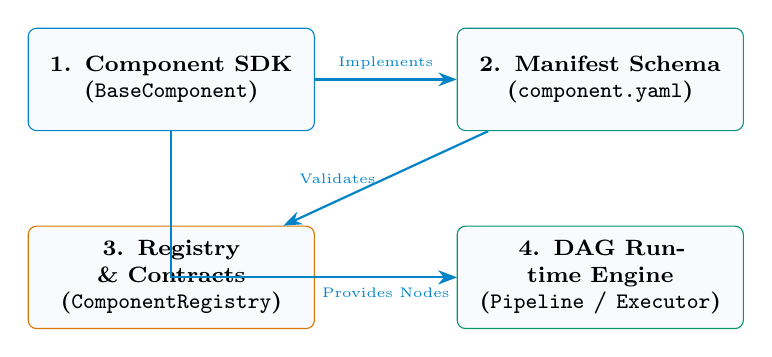
\begin{tikzpicture}[
    node distance=1.2cm and 1.8cm,
    block/.style={rectangle, draw=brandnavy, fill=bglight, rounded corners=3pt, text width=3.4cm, minimum height=1.3cm, align=center, font=\footnotesize\bfseries},
    edge/.style={->, >=Stealth, thick, color=brandblue}
]
    \node[block, draw=brandblue] (sdk) {1. Component SDK\\(\texttt{BaseComponent})};
    \node[block, right=of sdk, draw=brandteal] (manifest) {2. Manifest Schema\\(\texttt{component.yaml})};
    \node[block, below=of sdk, draw=brandamber] (registry) {3. Registry \& Contracts\\(\texttt{ComponentRegistry})};
    \node[block, below=of manifest, draw=brandemerald] (runtime) {4. DAG Runtime Engine\\(\texttt{Pipeline} / \texttt{Executor})};

    \draw[edge] (sdk) -- node[above, font=\tiny\color{mutedgray}]{Implements} (manifest);
    \draw[edge] (manifest) -- node[left, font=\tiny\color{mutedgray}]{Validates} (registry);
    \draw[edge] (registry) -- node[below, font=\tiny\color{mutedgray}]{Provides Nodes} (runtime);
    \draw[edge] (sdk) |- (runtime);
\end{tikzpicture}
\caption{The Four Decoupled Subsystems of the FinForge AI Framework.}
\label{fig:four_pillars}
\end{figure}

\subsection{Pillar I: Component SDK \& Lifecycle Contract}
Every algorithmic component in FinForge subclasses \texttt{BaseComponent} (\texttt{finforge.component}). The component lifecycle adheres to a deterministic, non-reversible state machine:

\begin{figure}[h!]
\centering
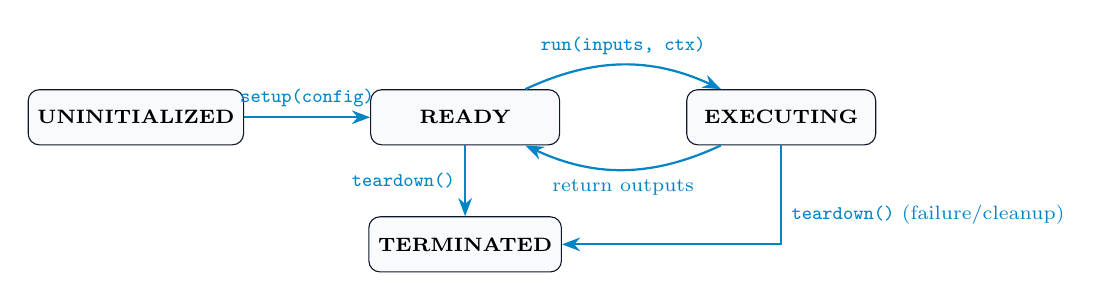
\begin{tikzpicture}[
    state/.style={rectangle, draw=brandnavy, fill=bglight, rounded corners=4pt, font=\scriptsize\bfseries, minimum width=2.4cm, minimum height=0.7cm},
    trans/.style={->, >=Stealth, thick, color=brandblue, font=\scriptsize}
]
    \node[state] (uninit) {UNINITIALIZED};
    \node[state, right=1.6cm of uninit] (ready) {READY};
    \node[state, right=1.6cm of ready] (exec) {EXECUTING};
    \node[state, below=0.9cm of ready] (term) {TERMINATED};

    \draw[trans] (uninit) -- node[above]{\texttt{setup(config)}} (ready);
    \draw[trans] (ready) edge[bend left=25] node[above]{\texttt{run(inputs, ctx)}} (exec);
    \draw[trans] (exec) edge[bend left=25] node[below]{return outputs} (ready);
    \draw[trans] (ready) -- node[left]{\texttt{teardown()}} (term);
    \draw[trans] (exec) |- node[below right, pos=0.25]{\texttt{teardown()} (failure/cleanup)} (term);
\end{tikzpicture}
\caption{Deterministic Three-Stage Component Lifecycle State Machine.}
\label{fig:lifecycle}
\end{figure}

\begin{itemize}[leftmargin=1.5em, itemsep=2pt]
    \item \texttt{setup(config: dict[str, Any]) -> None}: Called once prior to pipeline evaluation. Allocates memory buffers, loads local weights, and validates required configuration keys. Raises \texttt{ComponentConfigurationError} on failure.
    \item \texttt{run(inputs: dict[str, Any], context: dict[str, Any]) -> dict[str, Any]}: Pure algorithmic execution. Consumes declared input ports and execution context, returning typed output ports. Raises \texttt{ComponentLifecycleError} if called before \texttt{setup()}, or \texttt{ComponentExecutionError} upon algorithmic failure.
    \item \texttt{teardown() -> None}: Idempotent resource disposal hook. Releases memory buffers, file handles, or network sockets. Safe to invoke multiple times.
\end{itemize}

\subsection{Pillar II: Declarative Component Manifests (\texttt{component.yaml})}
FinForge enforces total separation between metadata and implementation. Component manifests are parsed via strict Pydantic v2 schemas (\texttt{finforge.manifest}) with \texttt{extra="forbid"}.

\begin{lstlisting}[language=yaml, caption={Production Component Manifest Definition (\texttt{component.yaml})}]
format_version: "1"
name: "financial-bm25-retriever"
version: "0.1.0"
description: "Scratch-built BM25 term weighting ranker for financial filings"
category: "rag"
entrypoint: "financial_retriever.component:BM25RetrieverComponent"

inputs:
  corpus_chunks:
    type: "array"
    required: true
    description: "Array of parsed document chunks"
  query_string:
    type: "string"
    required: true
    description: "Financial query or investigative prompt"

outputs:
  top_passages:
    type: "array"
    description: "Ranked relevant text passages"
  relevance_scores:
    type: "array"
    description: "Robertson-Sparck Jones BM25 similarity scores"

config:
  k1:
    type: "float"
    default: 1.5
    description: "Term frequency saturation parameter"
  b:
    type: "float"
    default: 0.75
    description: "Document length normalization penalty"
  top_k:
    type: "integer"
    default: 3
    description: "Maximum number of passages to return"
\end{lstlisting}

\subsection{Pillar III: Pipeline Graph Engine \& Static Invariants}
Workflows in FinForge AI are modeled as Directed Acyclic Graphs (DAGs) (\texttt{finforge.pipeline.graph.PipelineGraph}). Structural integrity is verified at assembly time prior to any runtime instantiation:
\begin{enumerate}[leftmargin=1.5em, itemsep=2pt]
    \item \textbf{Acyclicity Guarantee}: Cycle detection is performed using depth-first search traversal; cycles immediately abort graph compilation with \texttt{CycleDetectedError}.
    \item \textbf{Static Port Compatibility}: Connections between producer output ports and consumer input ports are checked against semantic type schemas (e.g., \texttt{integer} safely promotes to \texttt{float}, but \texttt{float} cannot narrow to \texttt{integer}). Missing ports raise \texttt{PortNotFoundError}.
    \item \textbf{Deterministic Topological Resolution}: Execution sequence is computed via Kahn's algorithm with min-heap tie-breaking, ensuring exact deterministic repeatability across execution environments.
\end{enumerate}

\subsection{Pillar IV: Runtime Execution \& Teardown Guarantees}
The \texttt{LocalSynchronousExecutor} runs pipelines locally and sequentially:
\begin{itemize}[leftmargin=1.5em, itemsep=2pt]
    \item Dynamically instantiates component instances based on manifest entrypoints.
    \item Resolves inputs from upstream node outputs combined with user external parameters.
    \item Enforces strict input validation before \texttt{run()} and output validation after \texttt{run()}.
    \item \textbf{Guaranteed Teardown}: Wraps execution in comprehensive \texttt{try...finally} constructs. Even if a downstream component crashes, all previously initialized upstream components are guaranteed clean \texttt{teardown()} invocations.
\end{itemize}

% ------------------------------------------------------------------------------
% SECTION 3: REAL-WORLD WORKING EXAMPLES
% ------------------------------------------------------------------------------
\section{End-to-End Practical Implementations}

\subsection{Example 1: First-Principles Financial RAG Pipeline}
This pipeline demonstrates a complete Retrieval-Augmented Generation workflow constructed entirely from first principles without LangChain or external vector stores.

\begin{figure}[h!]
\centering
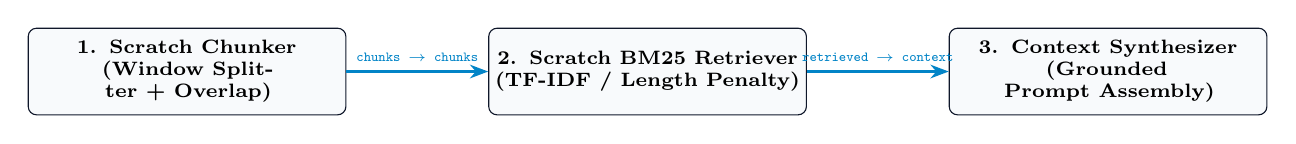
\begin{tikzpicture}[
    node distance=1.2cm and 1.8cm,
    block/.style={rectangle, draw=brandnavy, fill=bglight, rounded corners=3pt, text width=3.8cm, minimum height=1.1cm, align=center, font=\scriptsize\bfseries},
    edge/.style={->, >=Stealth, thick, color=brandblue}
]
    \node[block] (chunker) {1. Scratch Chunker\\(Window Splitter + Overlap)};
    \node[block, right=of chunker] (bm25) {2. Scratch BM25 Retriever\\(TF-IDF / Length Penalty)};
    \node[block, right=of bm25] (synth) {3. Context Synthesizer\\(Grounded Prompt Assembly)};

    \draw[edge] (chunker) -- node[above, font=\tiny\color{brandnavy}]{\texttt{chunks $\rightarrow$ chunks}} (bm25);
    \draw[edge] (bm25) -- node[above, font=\tiny\color{brandnavy}]{\texttt{retrieved $\rightarrow$ context}} (synth);
\end{tikzpicture}
\caption{Topological DAG for Pure Scratch-Built RAG Pipeline.}
\label{fig:rag_dag}
\end{figure}

\begin{lstlisting}[language=Python, caption={Scratch BM25 Component Implementation in FinForge}]
import math, re
from typing import Any
from finforge.component import BaseComponent

class ScratchBM25RetrieverComponent(BaseComponent):
    """Calculates Robertson-Sparck Jones BM25 relevance scores."""

    def setup(self, config: dict[str, Any]) -> None:
        self._top_k = int(config.get("top_k", 2))
        self._k1 = float(config.get("k1", 1.5))
        self._b = float(config.get("b", 0.75))

    @staticmethod
    def _tokenize(text: str) -> list[str]:
        return re.findall(r"\w+", text.lower())

    def run(self, inputs: dict[str, Any], context: dict[str, Any]) -> dict[str, Any]:
        chunks: list[str] = inputs["chunks"]
        query: str = inputs["query"]
        q_tokens = self._tokenize(query)

        N = len(chunks)
        doc_tokens = [self._tokenize(c) for c in chunks]
        avgdl = sum(len(dt) for dt in doc_tokens) / max(1, N)

        # Compute document frequencies
        df: dict[str, int] = {}
        for dt in doc_tokens:
            for token in set(dt):
                df[token] = df.get(token, 0) + 1

        # Compute BM25 scores
        scores: list[tuple[float, str]] = []
        for i, dt in enumerate(doc_tokens):
            score = 0.0
            doc_len = len(dt)
            tf_map = {t: dt.count(t) for t in set(dt)}
            for q in q_tokens:
                if q in df:
                    idf = math.log((N - df[q] + 0.5) / (df[q] + 0.5) + 1.0)
                    tf = tf_map.get(q, 0)
                    denom = tf + self._k1 * (1 - self._b + self._b * (doc_len / avgdl))
                    score += idf * ((tf * (self._k1 + 1)) / max(0.001, denom))
            scores.append((score, chunks[i]))

        scores.sort(key=lambda x: x[0], reverse=True)
        return {"retrieved_chunks": [c for _, c in scores[:self._top_k]]}

    def teardown(self) -> None:
        pass
\end{lstlisting}

\subsection{Example 2: Financial Multi-Pillar Risk Analysis Pipeline}
The repository includes an active financial risk analysis pipeline connecting text normalization, Loughran-McDonald sentiment extraction, and 5-pillar risk tagging:

\begin{lstlisting}[language=yaml, caption={Financial Risk Analysis Pipeline Definition (\texttt{pipeline.yaml})}]
format_version: "1"
name: "financial-risk-analysis"
description: "Multi-stage financial risk and regulatory sentiment analyzer"

nodes:
  - id: "text_cleaner"
    component: "text-cleaner"
    config:
      lowercase: false
      strip_html: true
  - id: "sentiment_scorer"
    component: "sentiment-scorer"
    config:
      sentiment_threshold: 0.1
  - id: "risk_tagger"
    component: "risk-tagger"
    config:
      risk_threshold: 50.0

edges:
  - source_node: "text_cleaner"
    source_port: "cleaned_texts"
    destination_node: "sentiment_scorer"
    destination_port: "texts"
  - source_node: "sentiment_scorer"
    source_port: "sentiment_results"
    destination_node: "risk_tagger"
    destination_port: "sentiment_results"
  - source_node: "sentiment_scorer"
    source_port: "sentiment_summary"
    destination_node: "risk_tagger"
    destination_port: "sentiment_summary"
\end{lstlisting}

\subsection{Example 3: Scratch Classical ML Pipeline (Lloyd's K-Means)}
Demonstrates unsupervised machine learning with zero external dependencies (no scikit-learn). The pipeline normalizes financial volatility/valuation vectors and clusters them into distinct risk regimes:

\begin{lstlisting}[language=Python, caption={Pipeline Composition & Execution Script}]
from finforge.pipeline.builder import Pipeline
from finforge.registry import ComponentRegistry

# 1. Initialize registry and discover components
registry = ComponentRegistry()
registry.discover(search_paths=["components"])

# 2. Assemble Directed Acyclic Graph
pipeline = Pipeline("financial-clusterer", registry=registry)
pipeline.add("scaler", "scratch-scaler", config={"with_std": True})
pipeline.add("kmeans", "scratch-kmeans", config={"k": 2, "max_iter": 50})
pipeline.add("evaluator", "scratch-profiler")

# 3. Establish dataflow edges
pipeline.connect("scaler", "scaled_features", "kmeans", "features")
pipeline.connect("kmeans", "labels", "evaluator", "labels")
pipeline.connect("kmeans", "centroids", "evaluator", "centroids")

# 4. Compile, validate, and execute
pipeline.validate()
result = pipeline.run(inputs={"scaler": {"features": [[12.5, 14.2], [42.0, 52.3]]}})
print(f"Status: {result.status.value} | Elapsed: {result.duration_ms:.2f}ms")
\end{lstlisting}

% ------------------------------------------------------------------------------
% SECTION 4: GAP ANALYSIS & STRATEGIC ROADMAP
% ------------------------------------------------------------------------------
\section{Gap Analysis: What Exists vs. What You Need to Add}

\subsection{Current Implementation Inventory}
The codebase currently contains **323 passing unit and integration tests** verifying core subsystems:
\begin{itemize}[leftmargin=1.5em, itemsep=2pt]
    \item \checkmark\ \textbf{Universal Base Contract}: \texttt{BaseComponent} lifecycle state machine and exception hierarchy.
    \item \checkmark\ \textbf{Strict Manifest Parser}: Pydantic v2 \texttt{ComponentManifest} with \texttt{extra="forbid"}.
    \item \checkmark\ \textbf{Contract Compatibility Engine}: Static port type compatibility and runtime schema validation.
    \item \checkmark\ \textbf{In-Memory Registry}: Local catalog with collision detection and discovery walkers.
    \item \checkmark\ \textbf{DAG Pipeline Engine}: Graph cycle detection, Kahn topological sort, serialization to/from YAML.
    \item \checkmark\ \textbf{CLI Developer Suite}: Typer commands (\texttt{create}, \texttt{create-pipeline}, \texttt{inspect}, \texttt{export}, \texttt{test}).
\end{itemize}

\subsection{Engineering Gap Analysis \& Strategic Roadmap}

\begin{table}[h!]
\centering
\small
\begin{tabularx}{\textwidth}{p{3.2cm} p{1.8cm} p{2.2cm} X}
\toprule
\textbf{Subsystem / Feature} & \textbf{Target Phase} & \textbf{Complexity} & \textbf{Functional Specification \& Scope} \\
\midrule
\textbf{CLI Pipeline Runner} & Immediate (v0.1.1) & Low (1-2 days) & Add \texttt{finforge run <pipeline.yaml> --inputs <file.json>} to invoke pipelines directly from terminal. \\
\textbf{Asynchronous DAG Executor} & Phase 1 (v0.2.0) & Medium (1 week) & Implement \texttt{AsyncExecutor} to execute independent branches concurrently via \texttt{asyncio.gather}. \\
\textbf{Hierarchical Config Subsystem} & Phase 1 (v0.2.0) & Medium (3-4 days) & Support cascading configuration resolution: \texttt{component.yaml} $\rightarrow$ \texttt{pipeline.yaml} $\rightarrow$ \texttt{.env} $\rightarrow$ CLI flags. \\
\textbf{Streaming Port Protocol} & Phase 2 (v0.3.0) & Medium (1 week) & Support Python generator yield protocols (\texttt{Generator[str, None, None]}) for token-by-token LLM output streaming. \\
\textbf{Scratch Vector Index} & Phase 2 (v0.3.0) & Low (3 days) & First-principles in-memory vector index with Cosine, Euclidean, and Dot-Product distance metrics in NumPy. \\
\textbf{Interactive Visual Canvas} & Phase 3 (v0.4.0) & High (2-3 weeks) & Web-based drag-and-drop DAG builder (React Flow) with direct export to valid \texttt{pipeline.yaml}. \\
\textbf{Remote Component Hub} & Phase 4 (v1.0.0) & High (3-4 weeks) & Centralized package index allowing \texttt{finforge pull <author/component>} with cryptographic signature verification. \\
\bottomrule
\end{tabularx}
\caption{Detailed Implementation Roadmap: Prioritized Subsystems & Technical Scope.}
\label{tab:roadmap}
\end{table}

\begin{calloutbox}[Immediate Priority Action Items]
\begin{enumerate}[leftmargin=1.2em, itemsep=2pt]
    \item \textbf{Implement \texttt{finforge run}}: Bridge the CLI gap so users can test end-to-end workflows without writing custom Python harness scripts.
    \item \textbf{Add Branching / Conditional Nodes}: Introduce predicate router nodes allowing DAG execution paths to diverge based on upstream output values.
    \item \textbf{Expand First-Principles Library}: Add pure Python chunkers, BPE tokenizers, and self-attention blocks into the public \texttt{components/} library.
\end{enumerate}
\end{calloutbox}

% ------------------------------------------------------------------------------
% SECTION 5: MASTER CHEATSHEET & QUICK REFERENCE
% ------------------------------------------------------------------------------
\section{The Master FinForge Cheat Sheet}

\begin{cheatsheetcard}{1. CLI Command Quick Reference}
\small
\begin{tabularx}{\linewidth}{p{5.5cm} X}
\textbf{Command} & \textbf{Action Description} \\
\midrule
\texttt{finforge --version} & Displays current installed framework version. \\
\texttt{finforge create <name> --domain <dom>} & Scaffolds a compliant component package with tests and manifest. \\
\texttt{finforge create-pipeline <name>} & Scaffolds a new pipeline project with isolated components dir. \\
\texttt{finforge test <path/to/component>} & Runs 4-stage architectural validator, lifecycle checks, and pytest. \\
\texttt{finforge inspect <pipeline.yaml>} & Parses manifest, validates DAG topology, and prints execution order. \\
\texttt{finforge export <yaml> --format mermaid} & Emits visual Mermaid diagram markdown code for pipeline topology. \\
\texttt{finforge export <yaml> --format dot} & Emits Graphviz DOT format for rendering vector architecture diagrams. \\
\end{tabularx}
\end{cheatsheetcard}

\vspace{6pt}

\begin{cheatsheetcard}{2. Supported Manifest Data Types (\texttt{SUPPORTED\_PORT\_TYPES})}
\small
\begin{tabularx}{\linewidth}{p{3.2cm} p{2.8cm} X}
\textbf{Port Type Name} & \textbf{Python Native Type} & \textbf{Permissible Connections \& Promotion Rules} \\
\midrule
\texttt{"string"} & \texttt{str} & Exact match only. \\
\texttt{"integer"} & \texttt{int} & Safe automatic promotion to \texttt{"float"} or \texttt{"number"}. \\
\texttt{"float"} / \texttt{"number"} & \texttt{float} & Exact match; cannot narrow to \texttt{"integer"}. \\
\texttt{"boolean"} & \texttt{bool} & Exact match only. \\
\texttt{"array"} & \texttt{list} & Validates item element compatibility when specified. \\
\texttt{"object"} & \texttt{dict} & Key-value structured payload. \\
\texttt{"tensor"} & \texttt{numpy.ndarray} & Multidimensional numeric arrays. \\
\texttt{"dataframe"} & \texttt{pandas.DataFrame} & Tabular dataframes. \\
\texttt{"any"} & \texttt{typing.Any} & Unrestricted universal fallback port. \\
\end{tabularx}
\end{cheatsheetcard}

\vspace{6pt}

\begin{cheatsheetcard}{3. Python Builder API Quick Reference}
\small
\begin{tabularx}{\linewidth}{p{5.5cm} X}
\textbf{Method Call} & \textbf{Behavior} \\
\midrule
\texttt{reg.register(cls, manifest=m)} & Registers a component class with its explicit manifest instance. \\
\texttt{reg.discover(paths=[...])} & Traverses workspace directory tree to auto-discover \texttt{component.yaml}. \\
\texttt{pipe = Pipeline("name", reg)} & Initializes pipeline builder connected to component registry. \\
\texttt{pipe.add("node\_id", "comp", cfg)} & Adds an execution node referencing registered component. \\
\texttt{pipe.connect(s\_id, s\_p, d\_id, d\_p)} & Connects producer output port to consumer input port with type checking. \\
\texttt{pipe.validate()} & Verifies invariants: node existence, port existence, compatibility, acyclicity. \\
\texttt{pipe.execution\_order()} & Computes deterministic topological dependency sequence. \\
\texttt{pipe.run(inputs=\{...\})} & Executes workflow via synchronous executor; guarantees teardown. \\
\texttt{pipe.save("pipeline.yaml")} & Serializes DAG topology into standardized, portable YAML. \\
\texttt{Pipeline.load("pipe.yaml", reg)} & Deserializes YAML pipeline into executable Python graph object. \\
\end{tabularx}
\end{cheatsheetcard}

\vspace{6pt}

\begin{cheatsheetcard}{4. Exception Hierarchy \& Error Diagnosis}
\small
\begin{tabularx}{\linewidth}{p{4.5cm} X}
\textbf{Exception Class} & \textbf{Root Cause \& Diagnostic Resolution} \\
\midrule
\texttt{ComponentConfigurationError} & Raised in \texttt{setup()}; invalid or missing configuration values. \\
\texttt{ComponentLifecycleError} & Calling \texttt{run()} before \texttt{setup()}, or after \texttt{teardown()}. \\
\texttt{ComponentExecutionError} & Internal failure inside algorithmic logic during \texttt{run()}. \\
\texttt{PortNotFoundError} & Edge references an input or output port undeclared in \texttt{component.yaml}. \\
\texttt{PortIncompatibleError} & Producer output port type cannot be legally cast to consumer input port. \\
\texttt{CycleDetectedError} & Graph contains circular dependency feedback loop; DAG must be strictly forward. \\
\texttt{ContractValidationError} & Runtime payload received at port violates declared schema type boundary. \\
\end{tabularx}
\end{cheatsheetcard}

% ------------------------------------------------------------------------------
% SECTION 6: CONCLUSION
% ------------------------------------------------------------------------------
\section{Conclusion}
FinForge AI addresses the systemic brittleness of modern AI engineering by returning to first principles: **mechanical transparency, strict interface contracts, modular isolation, and deterministic execution**. By establishing a solid foundational architecture with comprehensive testing and zero-execution inspection, FinForge AI provides the ideal platform for building verifiable, production-grade intelligence from scratch.

\end{document}
